\paragraph{}
Nos dias atuais é quase impossível não utilizarmos um \textit{software}, seja ele o \textit{driver} que mostra o vídeo no \textit{display} do seu \textit{smartfone}, até a aplicação web que você utiliza para fazer compras online. Tudo contém um programa, ou um \textit{script} responsável, mesmo que não visível para o usuário. Porém, como você tem a permissão de utiliza-lo?

\paragraph{}
Sabe-se que para tudo na vida tem leis e regras, no mundo da computação não é diferente, há algo chamado licenças de \textit{software}, que são documentos através dos quais os detentores dos direitos sobre um programa de computador autorizam usos de seu trabalho que, de outra forma, estariam protegidos pelas leis vigentes no local \cite{sabino2009licenccas}. No caso do \textit{software} livre temos os 4 direitos básicos que o \textit{software} pode ser usado: copiado, estudado, modificado e redistribuído sem restrição \cite{fsf}. A forma usual de um \textit{software} ser distribuído livremente é sendo acompanhado por uma licença de \textit{software} livre (como a GPL ou a BSD), e com a disponibilização do seu código-fonte \cite{campos2006software}.

\paragraph{}
Ao pesquisar sobre licenças de \textit{software} livre é possível encontrar vários tipos para todos os casos, desde a mais permissiva até a mais proibitiva. Porém, qual o impacto de cada licença dentro do desenvolvimento de um \textit{software}? Para isso, o objetivo deste trabalho é utilizar o maior hub de código do mundo, atualmente o GitHub, para analisar o impacto de uma licença dentro de um projeto de código aberto e como isso afeta sua comunidade e contribuidores.

\paragraph{}
Inspirados pelo botão de redes sociais modernas, os usuários do GitHub também podem estrelar um repositório, presumivelmente para manifestar interesse ou satisfação com o projeto hospedado\cite{gousios2014exploratory, gousios2015work}. Por exemplo, os desenvolvedores podem separar sua própria cópia de um repositório, trabalhar e melhorar o código localmente e, em seguida, enviar uma solicitação pull para integrar as mudanças no repositório principal\cite{borges2016understanding}. Gerando assim uma popularidade de alguns projetos, e tirando esse proveito de semelhanças com redes sociais fica mais fácil poder analisar o que é tendencia ou não, já que os indices de cada projeto ja estão definidos por alguns indices mostrados na Figura \ref{fig:github-linux}
\begin{figure}[h!]
    \centering
    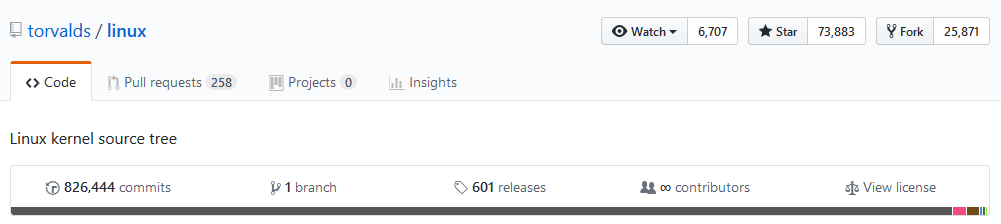
\includegraphics[width=\linewidth]{assets/images/github-linux.PNG}
    \caption{Exemplo de Repositório no Github (Kernel Linux)}
    \label{fig:github-linux}
\end{figure}

\paragraph{}
Este trabalho tem como objetivo estudar a rede de desenvolvedores Github em torno de seus repositórios aplicando técnicas de \textit{DataScience} para descobrir alguns \textit{KPI's (Key Performance Indicator)} usando informações públicas dos desenvolvedores disponíveis via API do GitHub.

% Colocar algum embasamento teórico aqui sobre o github
% Tambem colocar algo sobre como vamos analisar esse impacto, baseado no embasamento dito acima...